\documentclass[11pt,a4paper]{article}
\usepackage[utf8]{inputenc}
\usepackage[spanish]{babel}
\usepackage{amsmath}
\usepackage{amsfonts}
\usepackage{amssymb}
\usepackage{graphicx}
\usepackage{geometry}
\usepackage{fancyhdr}
\usepackage{enumitem}

% Configuración de márgenes
\geometry{left=2cm,right=2cm,top=2.5cm,bottom=2.5cm}

% Encabezado y pie de página
\pagestyle{fancy}
\fancyhf{}
\lhead{Asistente de IA - Física}
\rhead{Cinemática: MRU y MRUA}
\cfoot{Página \thepage}

\begin{document}

\begin{center}
    \LARGE \textbf{Guía de Ejercicios: Cinemática} \\
    \vspace{0.2cm}
    \large Resolución de Problemas y Análisis Gráfico
\end{center}

\vspace{0.5cm}

\section*{Instrucciones}
Lea atentamente cada enunciado y observe el gráfico adjunto. Resuelva utilizando las ecuaciones de movimiento correspondientes y verifique su resultado con la sección de respuestas al final.

\vspace{0.5cm}

% --- BLOQUE DE EJERCICIOS ---
% Este marcador será reemplazado por el script de Python
\subsection*{Ejercicio 1}
Determine la velocidad constante de un objeto que recorre desde 10.0 m hasta 582.0 m en un intervalo de 26.0 segundos.

\begin{center}
    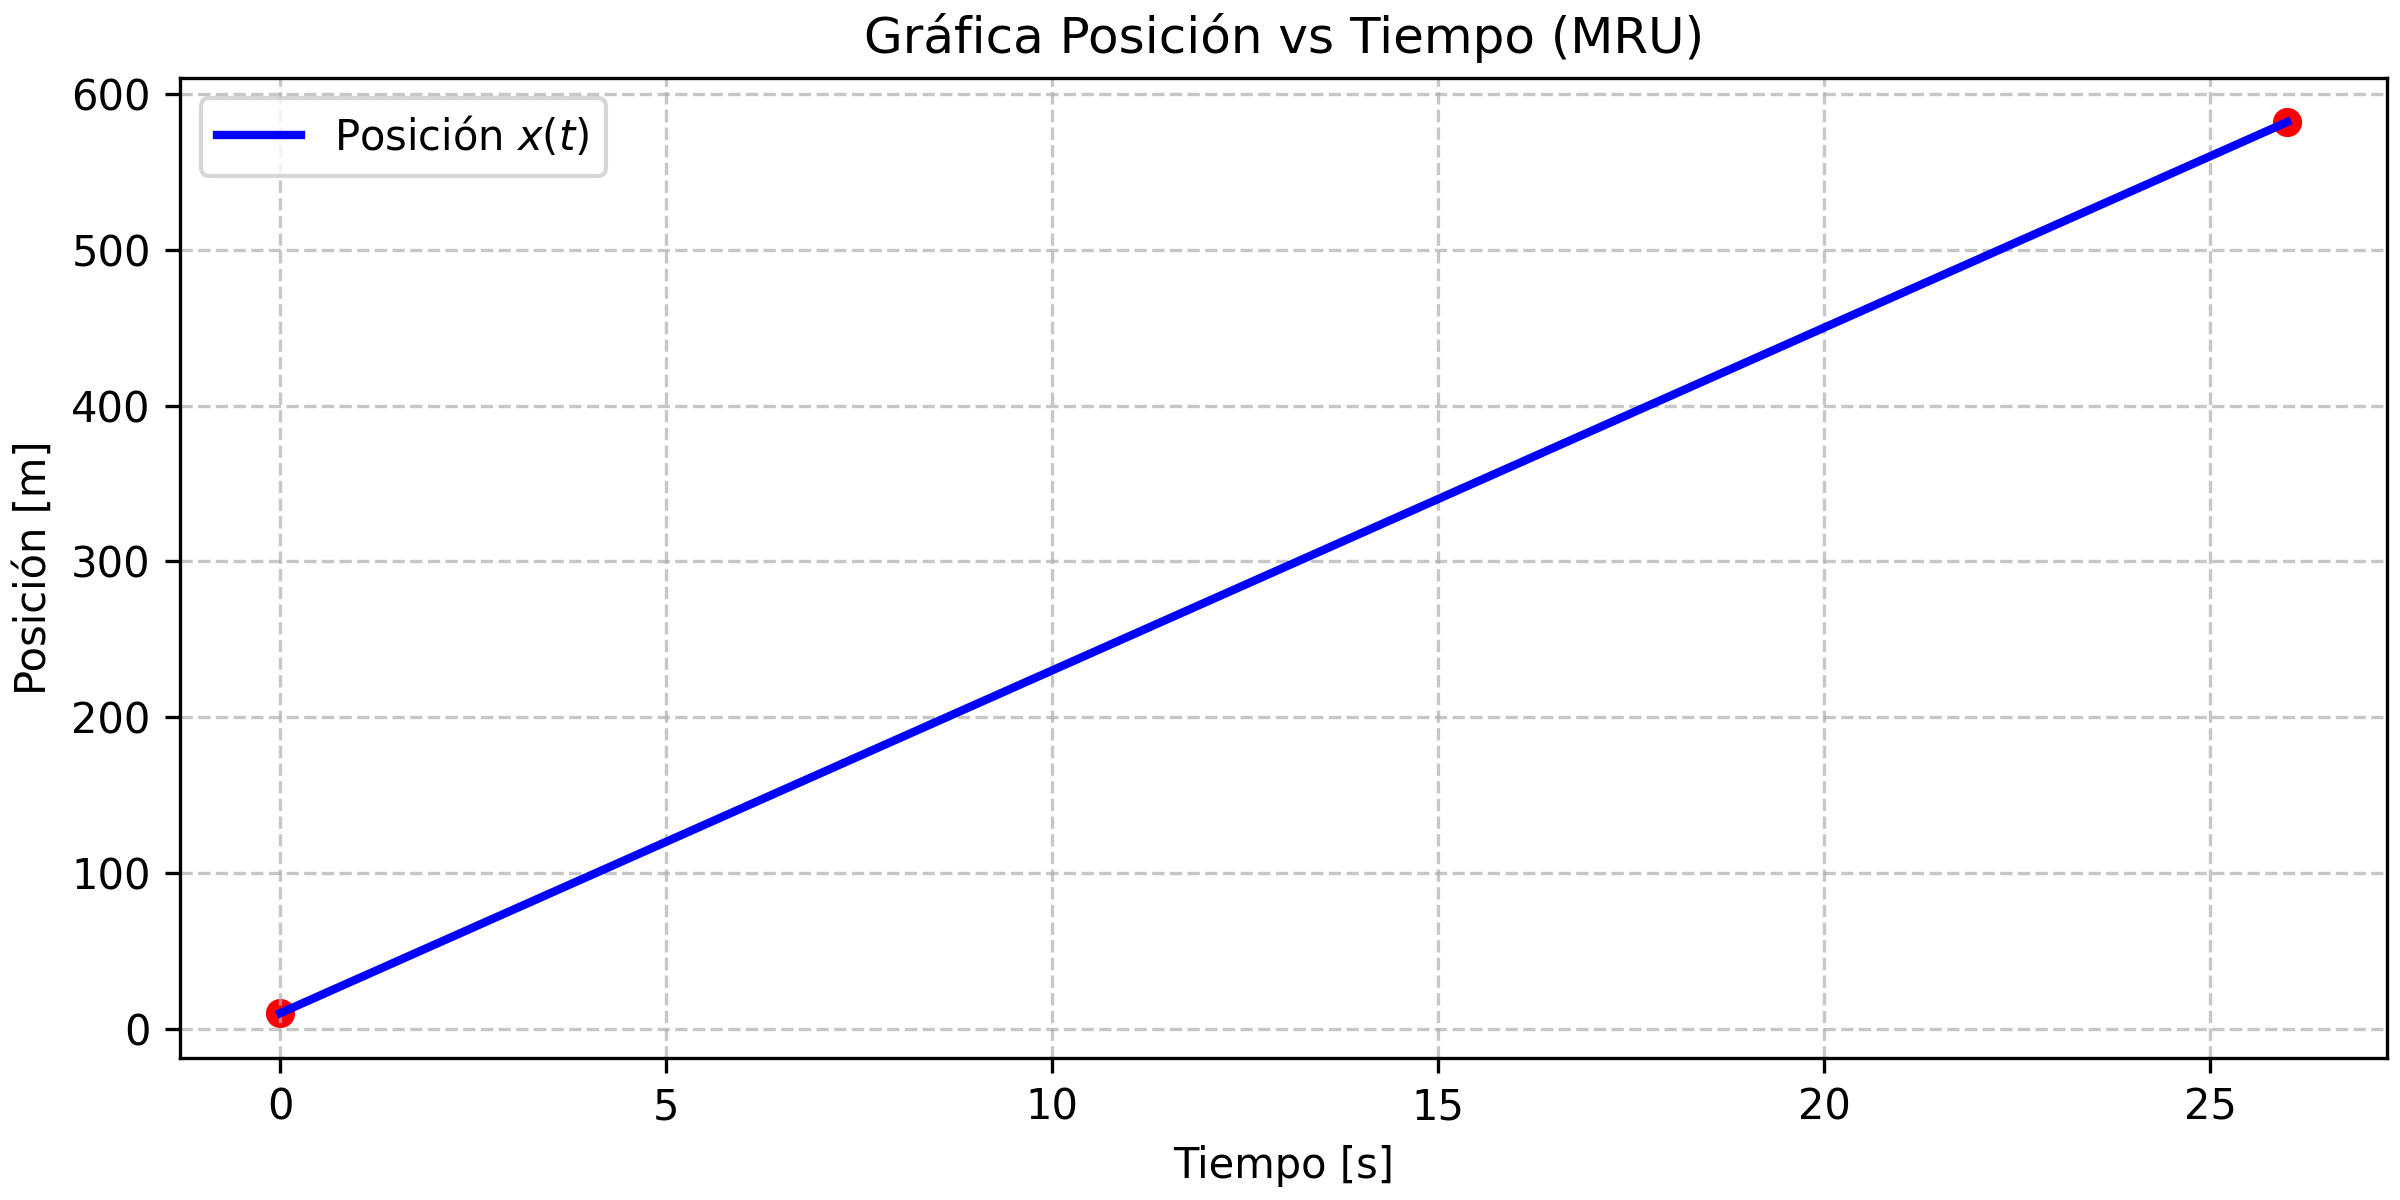
\includegraphics[width=0.8\textwidth]{grafico_1.png}
\end{center}

\vspace{0.5cm}
\textbf{Espacio para Resolución:}
\hrulefill
\vspace{1.5cm}
\hrulefill
\vspace{1.5cm}
\hrulefill
\vspace{1cm}

\subsection*{Ejercicio 2}
Un objeto inicia su movimiento a 22.0 m/s y alcanza una velocidad de 46.0 m/s en 3.0 segundos. Calcule su aceleración y la distancia total recorrida.

\begin{center}
    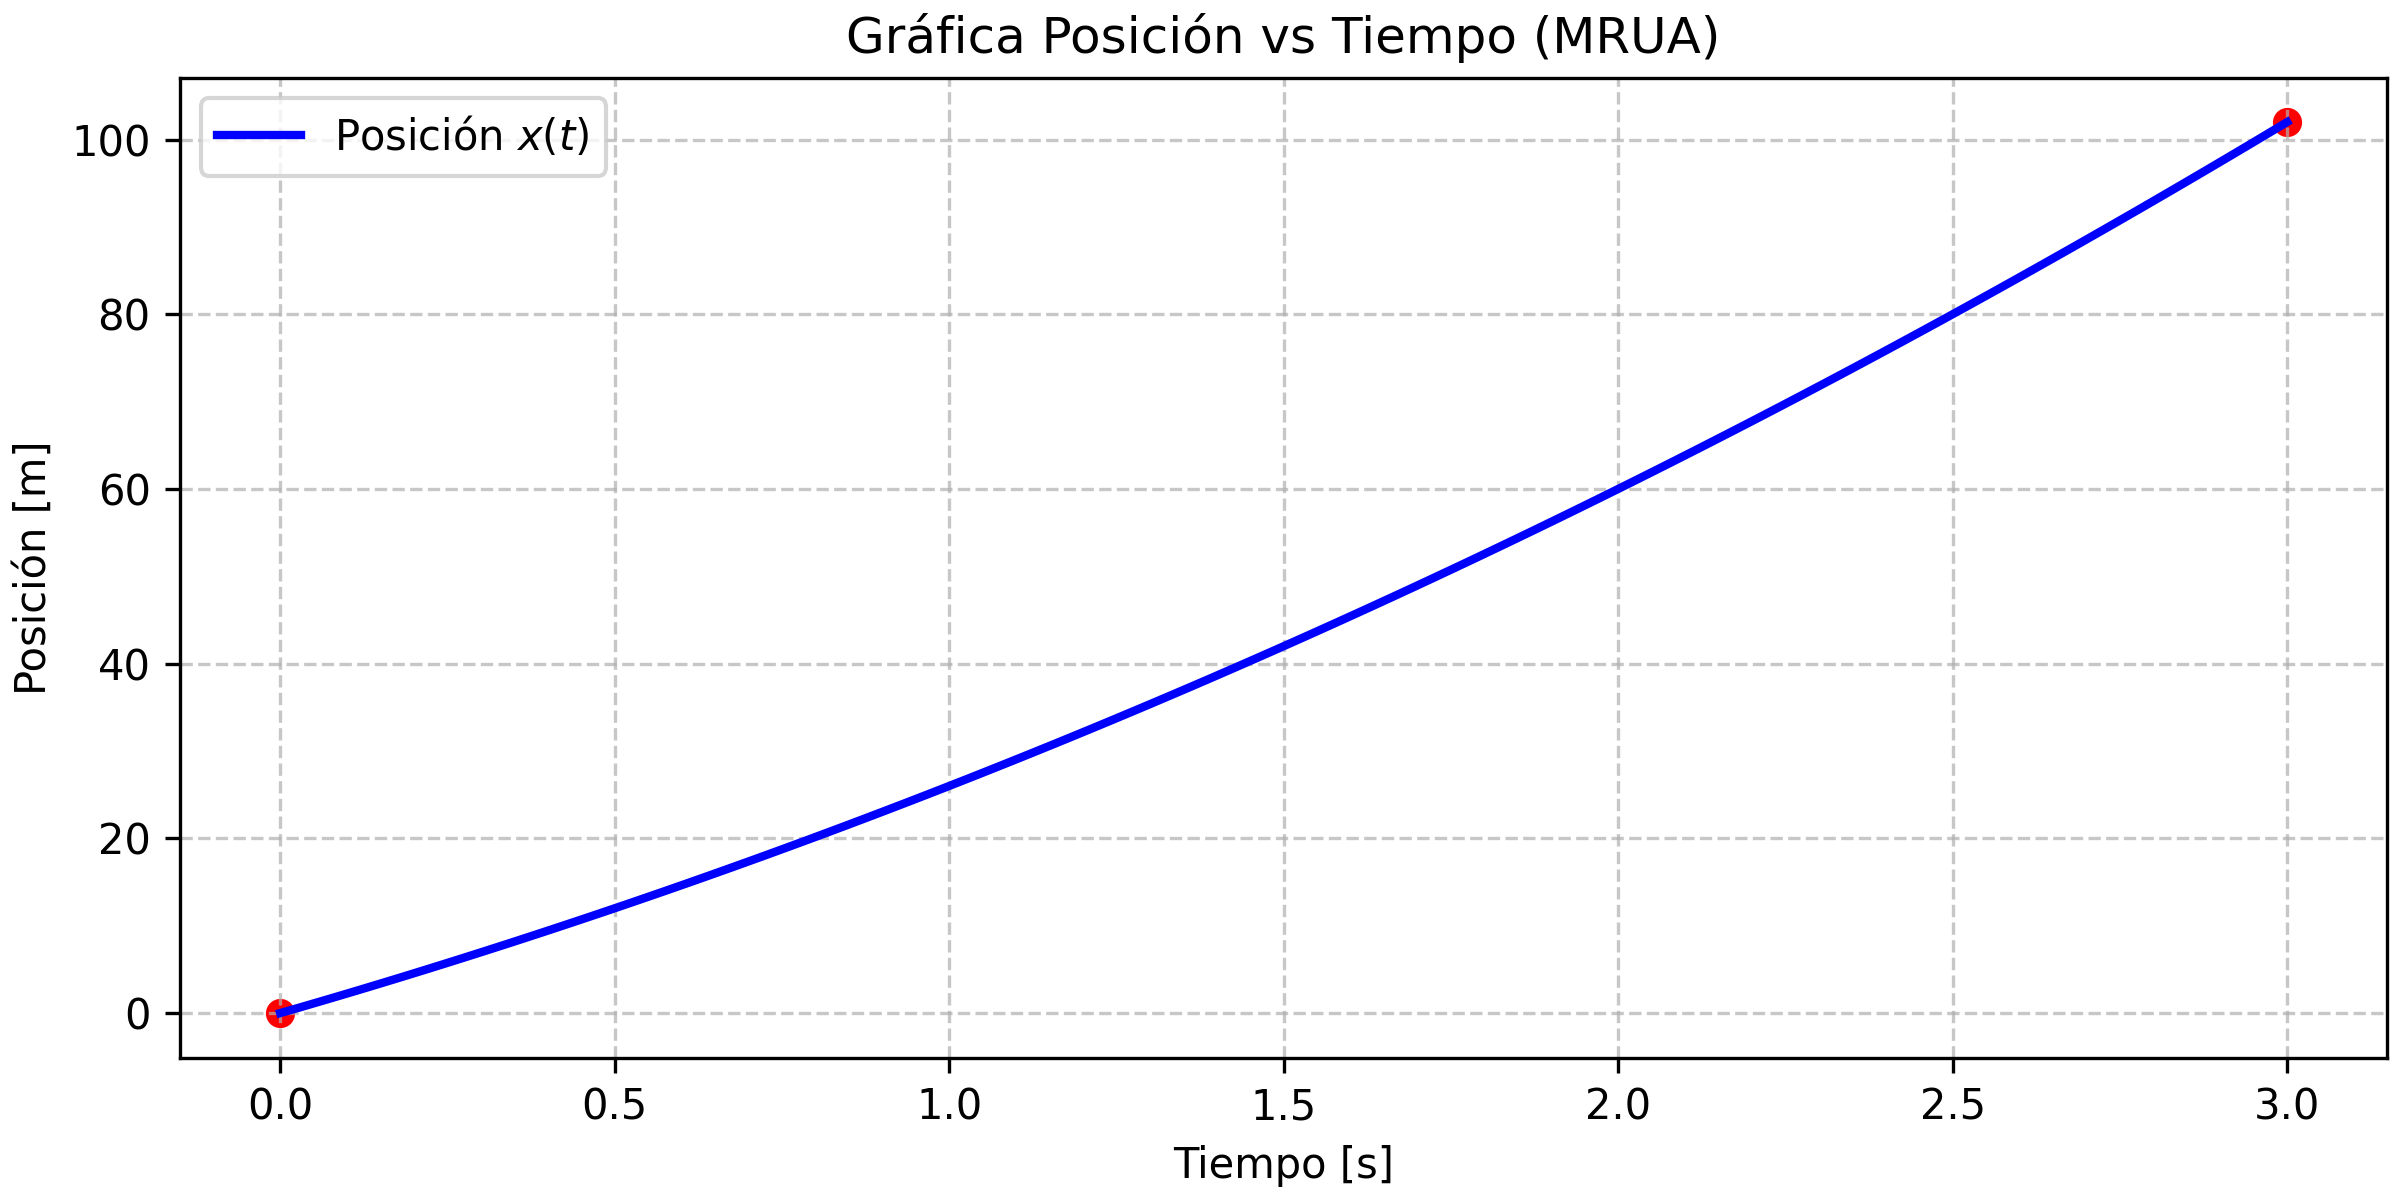
\includegraphics[width=0.8\textwidth]{grafico_2.png}
\end{center}

\vspace{0.5cm}
\textbf{Espacio para Resolución:}
\hrulefill
\vspace{1.5cm}
\hrulefill
\vspace{1.5cm}
\hrulefill
\vspace{1cm}

\subsection*{Ejercicio 3}
Dado el vector V = (-3.00, -7.00), calcule el vector resultante R = 5 * V (multiplicación por escalar).

\begin{center}
    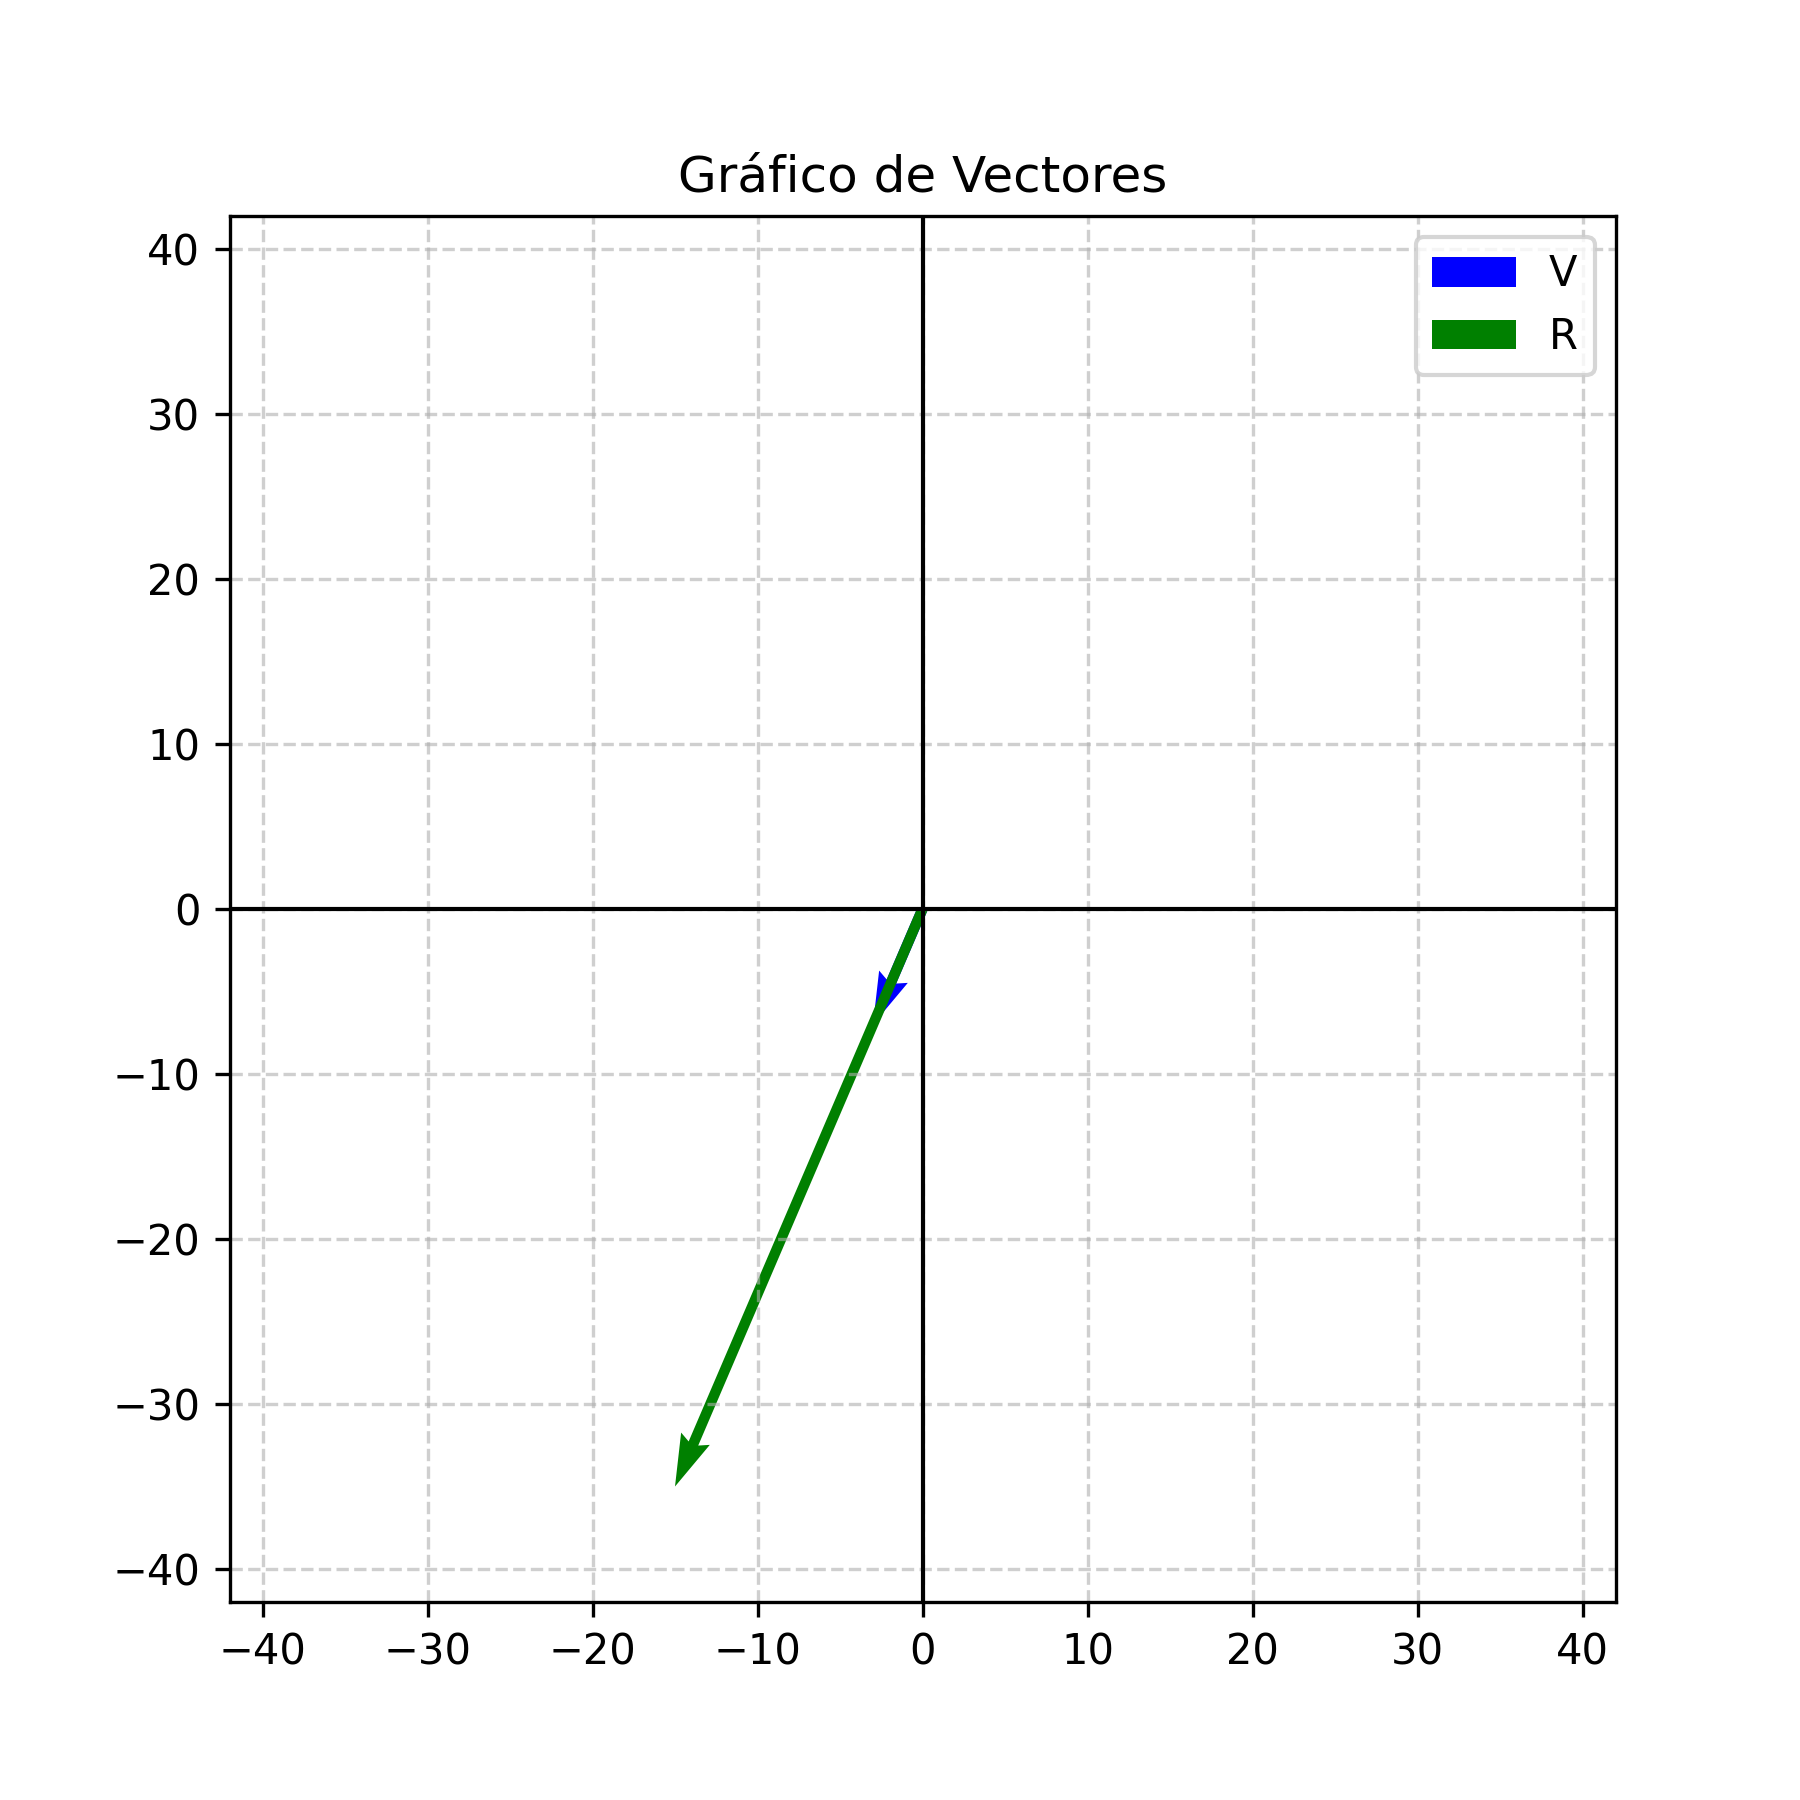
\includegraphics[width=0.8\textwidth]{grafico_3.png}
\end{center}

\vspace{0.5cm}
\textbf{Espacio para Resolución:}
\hrulefill
\vspace{1.5cm}
\hrulefill
\vspace{1.5cm}
\hrulefill
\vspace{1cm}

\subsection*{Ejercicio 4}
Encuentre la diferencia entre los vectores A = (2.00, 6.00) y B = (0.00, 4.00) (R = A - B). Grafique ambos vectores y el resultante.

\begin{center}
    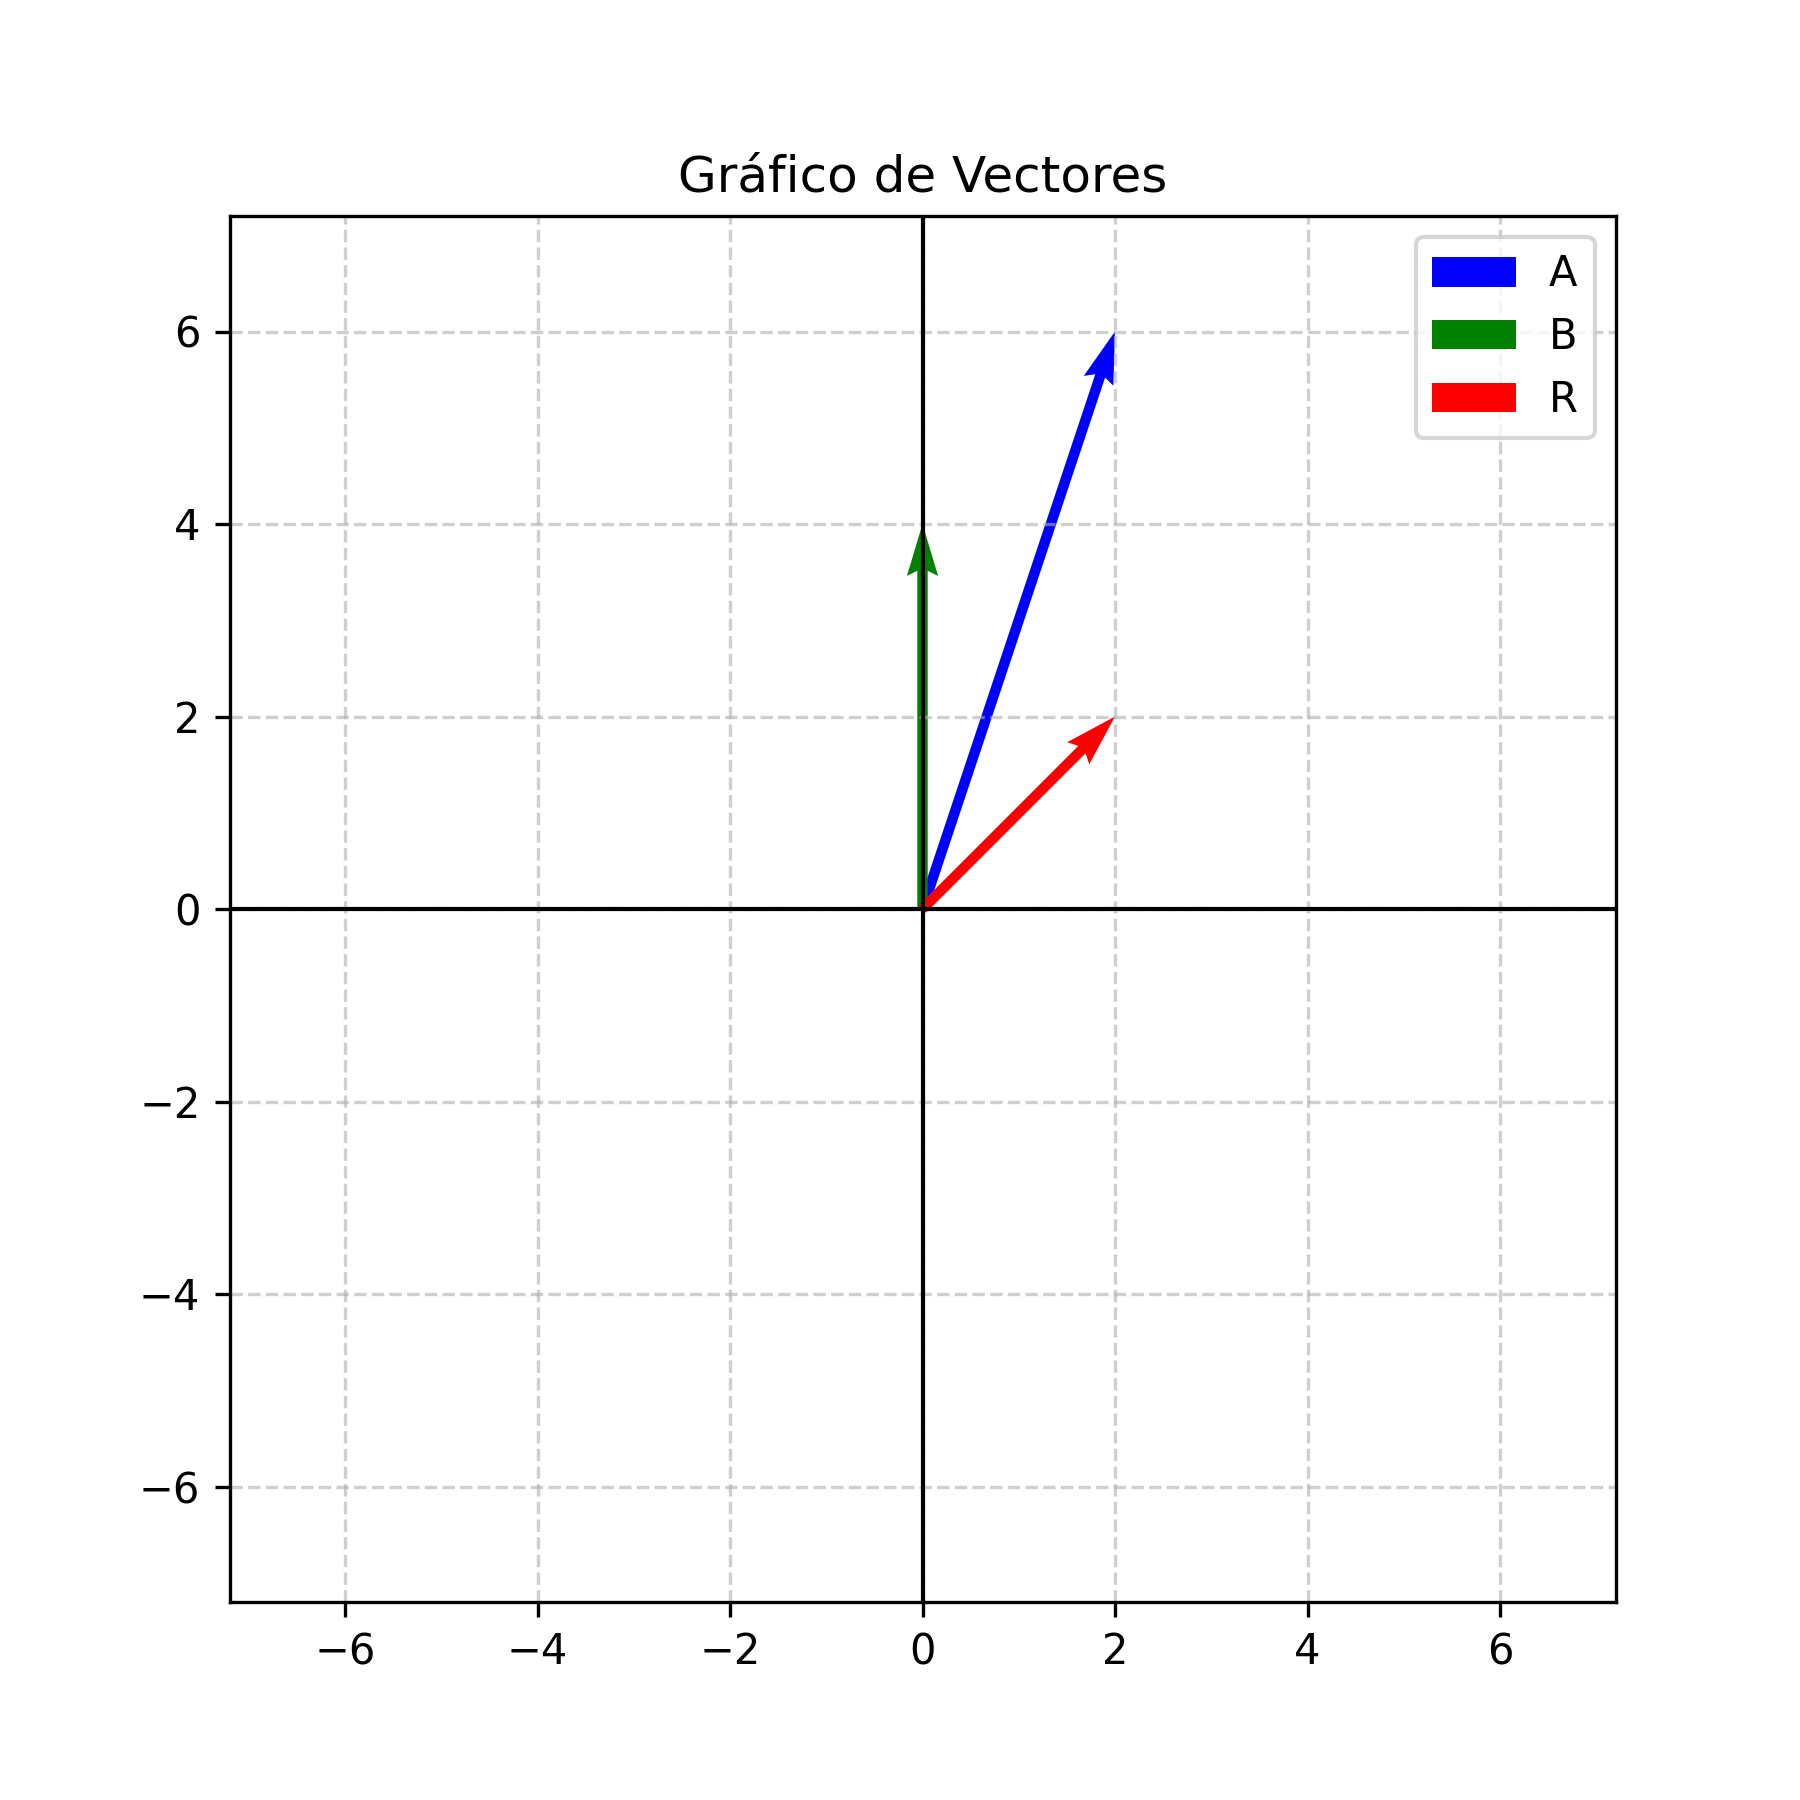
\includegraphics[width=0.8\textwidth]{grafico_4.png}
\end{center}

\vspace{0.5cm}
\textbf{Espacio para Resolución:}
\hrulefill
\vspace{1.5cm}
\hrulefill
\vspace{1.5cm}
\hrulefill
\vspace{1cm}


\newpage

% --- SECCIÓN DE RESPUESTAS ---
\section*{Clave de Respuestas}
A continuación se presentan los resultados numéricos para que puedas verificar tu trabajo:

\begin{enumerate}[label=\textbf{Ejercio \arabic*:}]
\item Posición Final: 582.00 m, Velocidad Final: 22.00 m/s

\item Posición Final: 102.00 m, Velocidad Final: 46.00 m/s

\item Vector R: (-15.00, -35.00), Magnitud: 38.08, Ángulo: 246.80°

\item Vector R: (2.00, 2.00), Magnitud: 2.83, Ángulo: 45.00°

\end{enumerate}

\end{document}
